\subsection{Analysis}
For the absorption curve we measured all the given aluminium plates with a caliper. 
The measured thickness of the different plates is found in the lab sheet in the appendix. 
An error of the scale of the caliper is $\pm0,05$\si{\mm}. 
Since this error is relatively small to the errors further in the experiment we neglected it.

Each plate got measured in the apparatus for 90 seconds giving us twelve counts $N_i$ with an corresponding error of $\pm\sqrt{N_i}$ for each different plate used.
This values are shown in Figure \ref{fig::absorb} with error bars.





\paragraph{Analysis method 1}
We determined from eye that after 3.5\si{\mm} the counted electrons are in the same range as the background noise picked up by the detector.
So we set our $x_{max}$ to 3.5mm with an estimated error of $\pm 0.25$\si{\mm}.


If we follow the last section described steps, we multiply the $x_{max}$ value with the given $\rho_{Al}$ ($2.69$\si{\g\centi\m}$^{-3}$) from the manual \cite{manual}.
This resulting value is then used to find the corresponding energy from the diagram \cite{manual}. 
Having a double logarithmic plot the error to read out the diagram is estimated half of the smallest grid drawn. 
In the range of $\rho_{Al} x_{max}= 941$\si{\mg\centi\m}$^{-2}$ the result for $E_{max}$ is $1.9 \pm 0.5$\si{\mega\electronvolt}.


Then we use this $E_{max}$ value to read the $E_{loss}$ from another table in the manual \cite{manual} giving us a loss energy of 108\si{\kilo\electronvolt}. 
This table used shows the energy loss of the electrons for 0.1mm stainless steel and has an scale of 4\si{\kilo\electronvolt}. 
Resulting in an reading error of $\pm$2\si{\kilo\electronvolt}. 
Ending in a $E_{maxsource}= E_{max}+E_{loss}= 2.0\pm0.5$\si{\mega\electronvolt}.
 


\paragraph{Analysis method 2}
In the second method we had to fit the from the manual \cite{manual} given model
\[
N(x)=N_0 e^{\mu x}
\]
to our values. 
This was done with the numpy polyfit method, retuning $\mu = 1.59$ with an given error of 0.07.
Using the given equation \cite{manual} to calculate 
\[
 E_max = \left(\frac{17\rho_{Al}}{\mu}\right)^{1/1.43} = 2.093,
\]
we only have to use the Gauss method on this equation to get the uncertainty on the maximum energy $\Delta E_{max} = 0.31$.
For the loss energy the same procedure as in method 1 is used.
Combined this results in  $E_{max}$ of $2.1 \pm 0,3$\si{\mega\electronvolt} and an $E_{maxsource}$ of  $2.2 \pm 0.3$\si{\mega\electronvolt}.



\paragraph{Analysis method 3}
For the last method we first had to subtract the background noise 
\[
N_{eff}=N-N_{BG}.
\]
This points are plotted as a function of $E_{max}-E(x)$ on a double logarithm scale as seen in figure \ref{fig::loglog}.


\begin{figure} [ht]
	\centering
	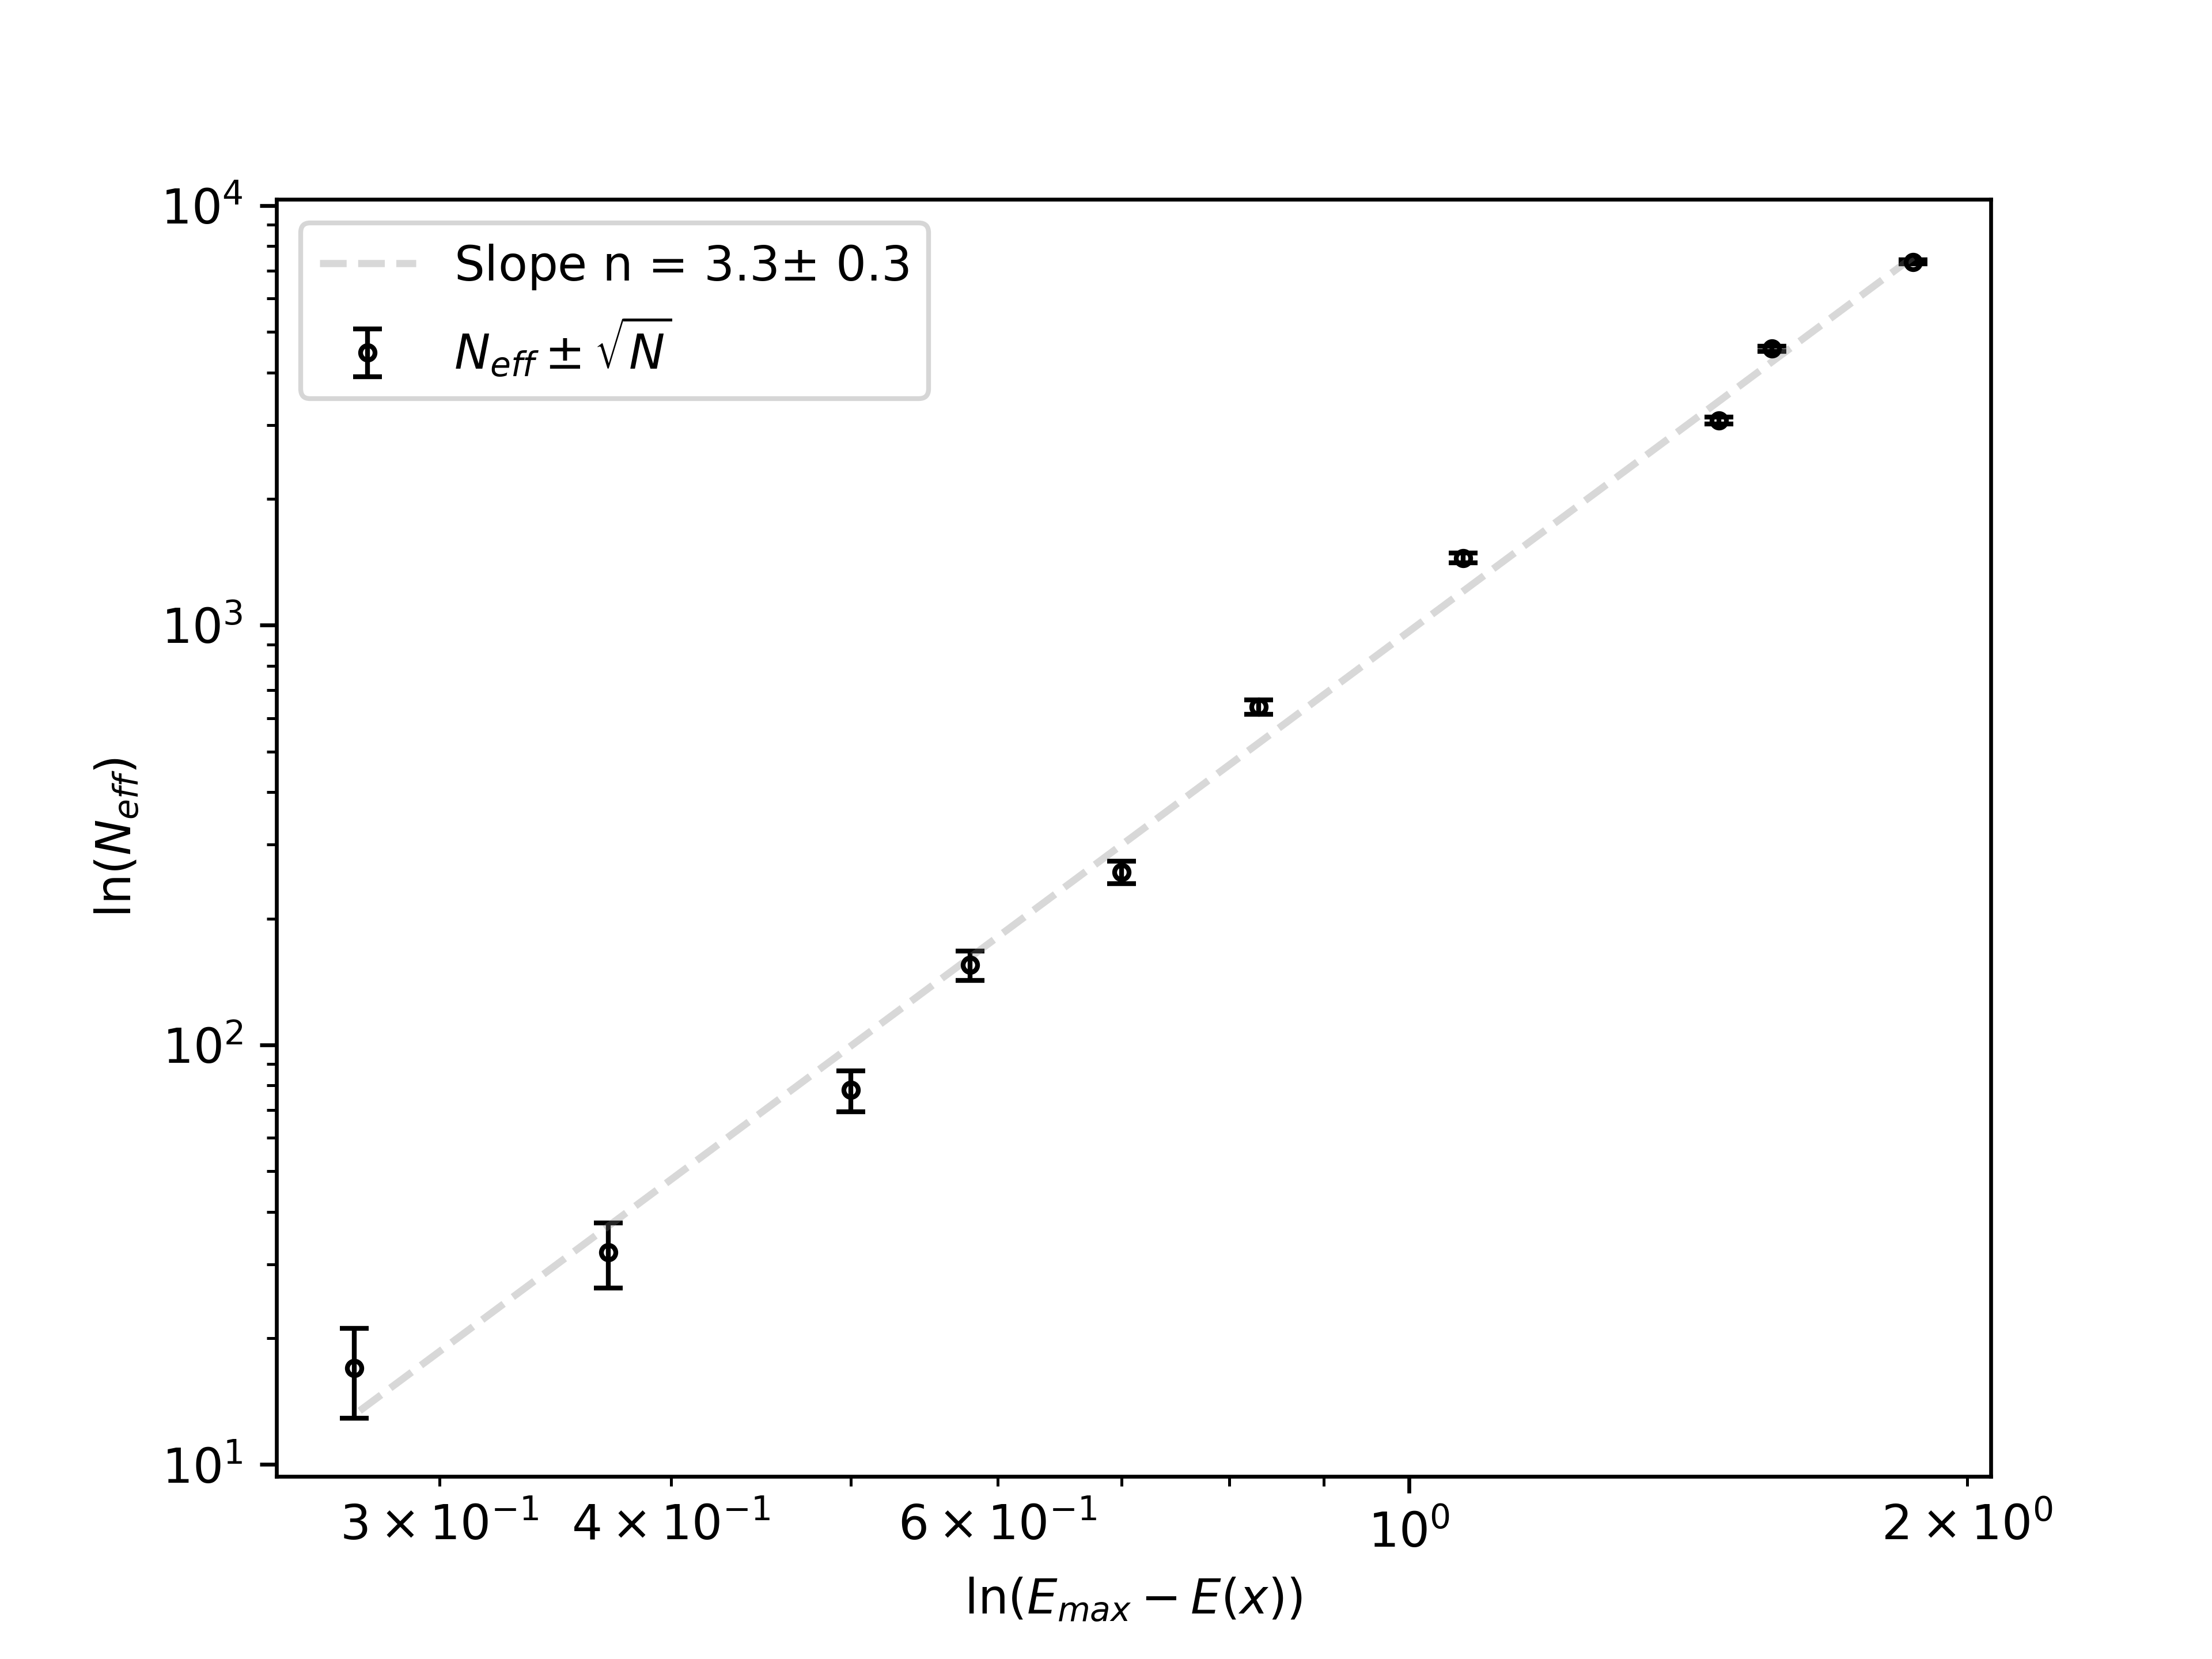
\includegraphics[width=400pt]{python/loglog.png}
	\caption{Number without background noise of counts per \SI{90}{\second} is double logarithmically plotted against the maximum energy from method 1 subtracted from the energies at the different sizes of the aluminium plates $E_{max}-E(x)$. Where is is the thickness of the plates in millimetre. Trough this point a linear fit is done with an slope value $n=3.3\pm0.3$. }
	\label{fig::loglog}
\end{figure}

From this point we determine the slope trough a polyfit in numpy.
This gives us an slope $n= 3.28$ and an error of $0.258$ which are used to generate the next plot.


Using this slope to calculate the values $N_{eff}^{1/n}$ and plotting it against the energy $E(x)$ as seen in figure \ref{fig::emax}.
The same procedure to find a slope is done again resulting in a linear model $f(E) = a + bE + \epsilon_E$.
The from the slope $b$ and offset $a$ we can calculate the function for $f(E)=0$.
Giving us the equation 
\[
E_{max} = \frac{-a}{b}
\]
with an already known error of 0,85, $a=15,21$ and $b=-8,14$ resulting in $E_{max}=1.9$ and the Gaussian error propagation we get an error of $\pm 0,3$\si{\mega\electronvolt}.


With the same approach like above  we get $E_{maxsource}=2.0 \pm 0.3$\si{\mega\electronvolt}.


\begin{figure} [ht]
	\centering
	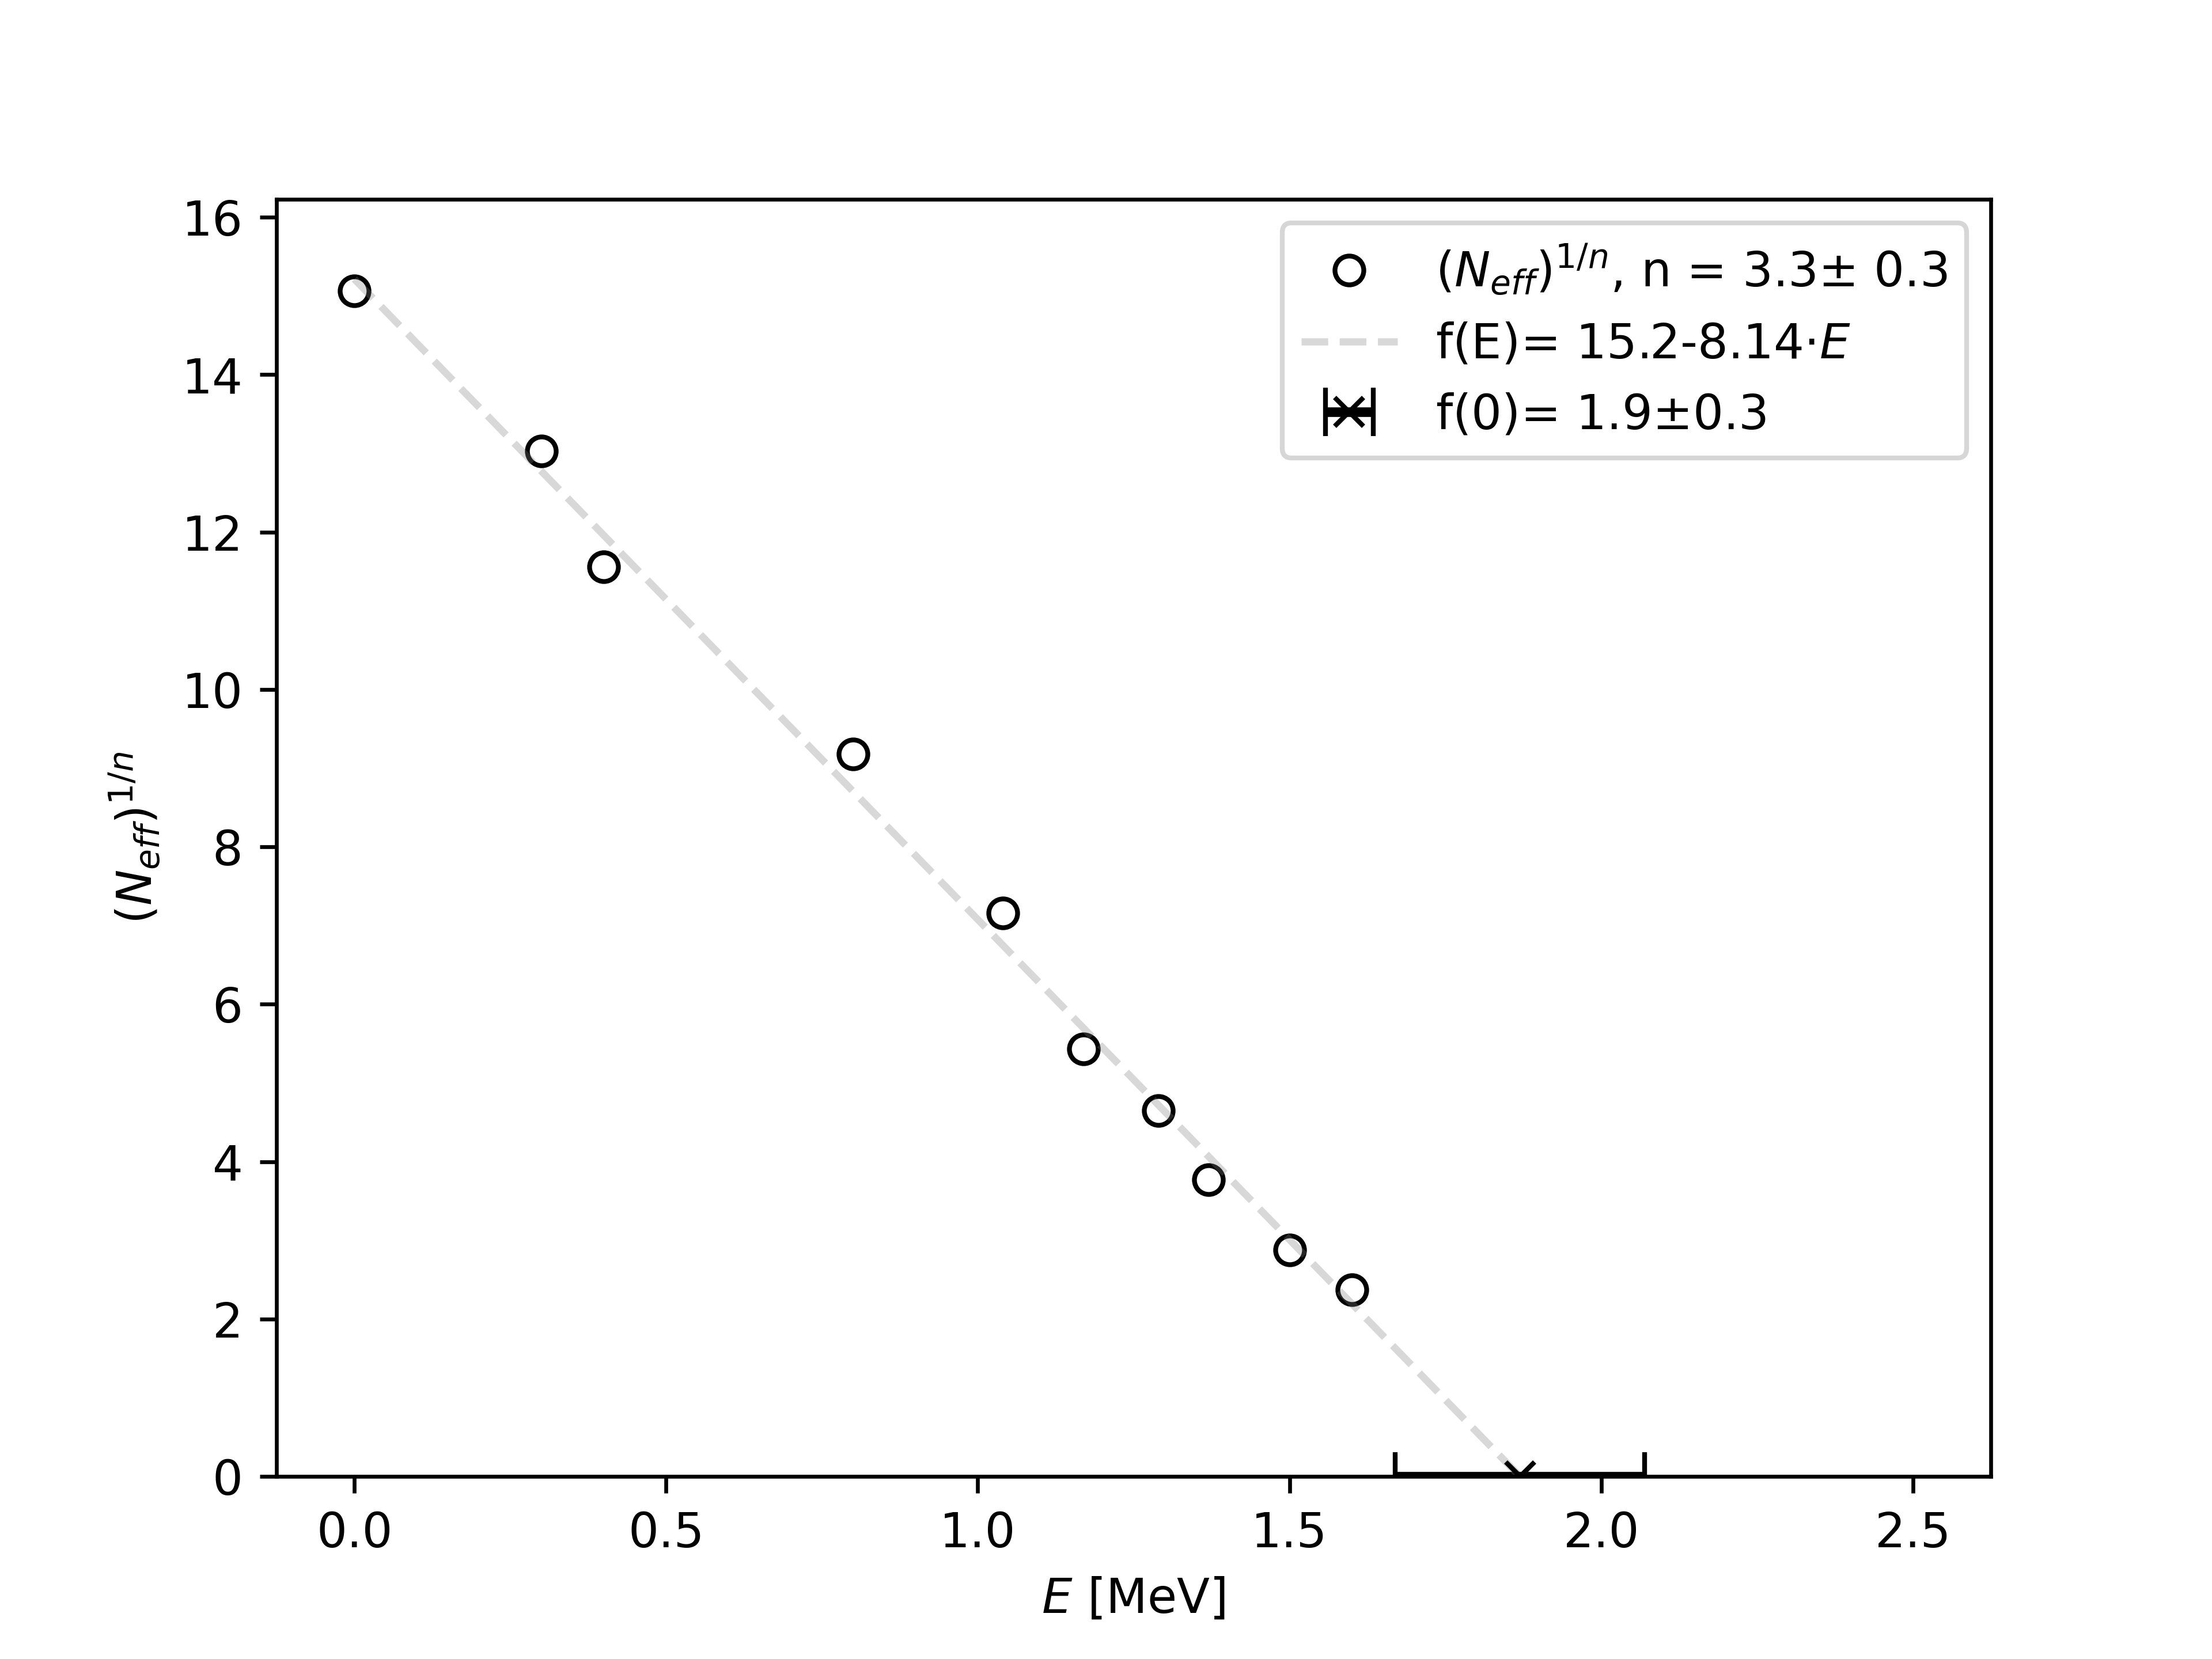
\includegraphics[width=400pt]{python/emax.png}
	\caption{Number of counts per \SI{90}{\second} is logarithmically plotted against the thickness of the aluminium plates [\si{\mm}]. The uncertainty of the counted numbers is displayed as error bars on the measured counts.}
	\label{fig::emax}
\end{figure}
